\documentclass{article}\usepackage[]{graphicx}\usepackage[]{color}
%% maxwidth is the original width if it is less than linewidth
%% otherwise use linewidth (to make sure the graphics do not exceed the margin)
\makeatletter
\def\maxwidth{ %
  \ifdim\Gin@nat@width>\linewidth
    \linewidth
  \else
    \Gin@nat@width
  \fi
}
\makeatother

\definecolor{fgcolor}{rgb}{0.345, 0.345, 0.345}
\newcommand{\hlnum}[1]{\textcolor[rgb]{0.686,0.059,0.569}{#1}}%
\newcommand{\hlstr}[1]{\textcolor[rgb]{0.192,0.494,0.8}{#1}}%
\newcommand{\hlcom}[1]{\textcolor[rgb]{0.678,0.584,0.686}{\textit{#1}}}%
\newcommand{\hlopt}[1]{\textcolor[rgb]{0,0,0}{#1}}%
\newcommand{\hlstd}[1]{\textcolor[rgb]{0.345,0.345,0.345}{#1}}%
\newcommand{\hlkwa}[1]{\textcolor[rgb]{0.161,0.373,0.58}{\textbf{#1}}}%
\newcommand{\hlkwb}[1]{\textcolor[rgb]{0.69,0.353,0.396}{#1}}%
\newcommand{\hlkwc}[1]{\textcolor[rgb]{0.333,0.667,0.333}{#1}}%
\newcommand{\hlkwd}[1]{\textcolor[rgb]{0.737,0.353,0.396}{\textbf{#1}}}%
\let\hlipl\hlkwb

\usepackage{framed}
\makeatletter
\newenvironment{kframe}{%
 \def\at@end@of@kframe{}%
 \ifinner\ifhmode%
  \def\at@end@of@kframe{\end{minipage}}%
  \begin{minipage}{\columnwidth}%
 \fi\fi%
 \def\FrameCommand##1{\hskip\@totalleftmargin \hskip-\fboxsep
 \colorbox{shadecolor}{##1}\hskip-\fboxsep
     % There is no \\@totalrightmargin, so:
     \hskip-\linewidth \hskip-\@totalleftmargin \hskip\columnwidth}%
 \MakeFramed {\advance\hsize-\width
   \@totalleftmargin\z@ \linewidth\hsize
   \@setminipage}}%
 {\par\unskip\endMakeFramed%
 \at@end@of@kframe}
\makeatother

\definecolor{shadecolor}{rgb}{.97, .97, .97}
\definecolor{messagecolor}{rgb}{0, 0, 0}
\definecolor{warningcolor}{rgb}{1, 0, 1}
\definecolor{errorcolor}{rgb}{1, 0, 0}
\newenvironment{knitrout}{}{} % an empty environment to be redefined in TeX

\usepackage{alltt}
\usepackage{amscd, amssymb, amsmath, verbatim, setspace}
\usepackage[left=1.0in, right=1.0in, top=1.0in, bottom=1.0in]{geometry}
\usepackage{mathrsfs}
\usepackage{listings}


\IfFileExists{upquote.sty}{\usepackage{upquote}}{}
\begin{document}
\begin{flushright}
Arif Ali\\
Math 611 Stochastic Simulation\\
Nov 17, 2016\\
\end{flushright}

\begin{center}
\LARGE\textbf{Homework 10}
  \end{center}
\section*{Exercise 1}
Please note the the joint density can be easily seperated:
\begin{equation}
\begin{split}
f(x,y) = \frac{x^{a+y-1}*e^{-(1+b)x}*b^{a}}{y!*\Gamma(a)} = \\
\frac{b^a}{\Gamma(a)}x^{a-1}e^{-bx}*\frac{x^{y}e^{-x}}{y!}
\end{split}
\end{equation}
From the reorganization of the joint density
\begin{equation}
f(x|y) = \frac{b^a}{\Gamma(a)}x^{a-1}e^{-bx} \sim gamma(a,b)
\end{equation}
Interesting to note that $f(x|y)$ does not depend on $y$, so in effect $f(x|y)=f(x)$.
\section*{Exercise 2}
From the reorganization of the joint density
\begin{equation}
f(y|x) = \frac{x^{y}e^{-x}}{y!}
\end{equation}
Which follows a poisson distribution where $\lambda=x$
\section*{Exercise 3}
\begin{knitrout}
\definecolor{shadecolor}{rgb}{0.969, 0.969, 0.969}\color{fgcolor}\begin{kframe}
\begin{alltt}
\hlstd{joint} \hlkwb{=} \hlkwa{function}\hlstd{(}\hlkwc{a}\hlstd{,}\hlkwc{b}\hlstd{)\{}
  \hlstd{x} \hlkwb{=} \hlkwd{rgamma}\hlstd{(}\hlnum{1}\hlstd{,a,b)}
  \hlstd{y} \hlkwb{=} \hlkwd{rpois}\hlstd{(}\hlnum{1}\hlstd{,x)}
  \hlkwd{return}\hlstd{(}\hlkwd{data.frame}\hlstd{(x,y,x}\hlopt{*}\hlstd{y))}
\hlstd{\}}
\end{alltt}
\end{kframe}
\end{knitrout}
\section*{Exercise 4}
\begin{knitrout}
\definecolor{shadecolor}{rgb}{0.969, 0.969, 0.969}\color{fgcolor}\begin{kframe}
\begin{alltt}
\hlstd{N} \hlkwb{=} \hlnum{5000}
\hlstd{prob_4} \hlkwb{=} \hlkwd{data.frame}\hlstd{(}\hlstr{"x"}\hlstd{,} \hlstr{"y"}\hlstd{,} \hlstr{"xy"}\hlstd{)[}\hlopt{-}\hlnum{1}\hlstd{,]}

\hlkwa{for}\hlstd{(t} \hlkwa{in} \hlnum{1}\hlopt{:}\hlstd{N)\{}
  \hlstd{prob_4} \hlkwb{=} \hlkwd{rbind}\hlstd{(prob_4,} \hlkwd{joint}\hlstd{(}\hlnum{1}\hlstd{,}\hlnum{1}\hlstd{))}
\hlstd{\}}
\hlkwd{names}\hlstd{(prob_4)} \hlkwb{=} \hlkwd{c}\hlstd{(}\hlstr{"x"}\hlstd{,} \hlstr{"y"}\hlstd{,} \hlstr{"xy"}\hlstd{)}
\hlstd{burn} \hlkwb{=} \hlnum{1e3}
\hlstd{sampled_gibbs} \hlkwb{=} \hlstd{prob_4[}\hlopt{-}\hlstd{(}\hlnum{1}\hlopt{:}\hlstd{burn),]}
\hlkwd{plot}\hlstd{(sampled_gibbs}\hlopt{$}\hlstd{x, sampled_gibbs}\hlopt{$}\hlstd{y,} \hlkwc{xlab} \hlstd{=} \hlstr{"x"}\hlstd{,} \hlkwc{ylab} \hlstd{=} \hlstr{"y"}\hlstd{)}
\end{alltt}
\end{kframe}
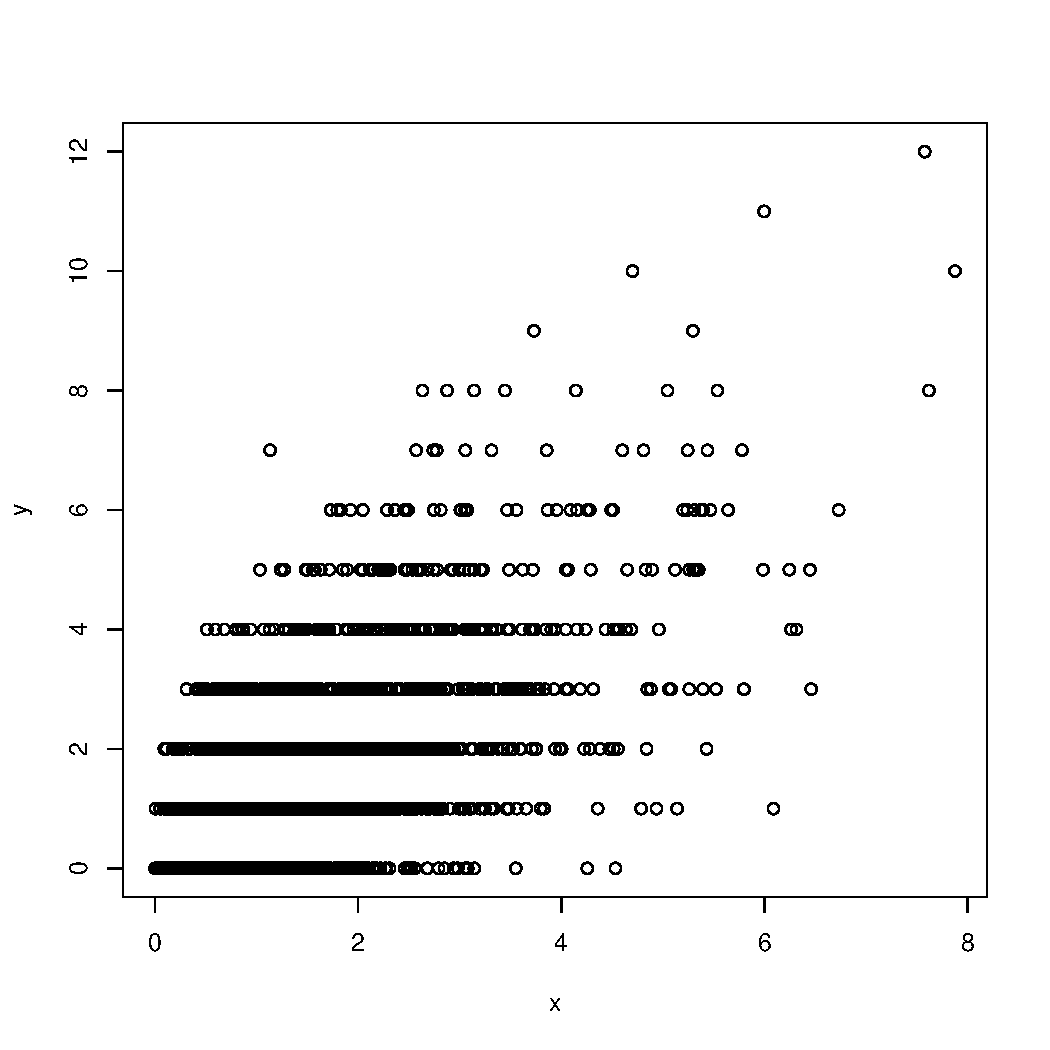
\includegraphics[width=0.60\linewidth]{figure/unnamed-chunk-3-1} 
\begin{kframe}\begin{alltt}
\hlkwd{hist}\hlstd{(sampled_gibbs}\hlopt{$}\hlstd{y,} \hlkwc{xlab} \hlstd{=} \hlstr{"y"}\hlstd{)}
\end{alltt}
\end{kframe}
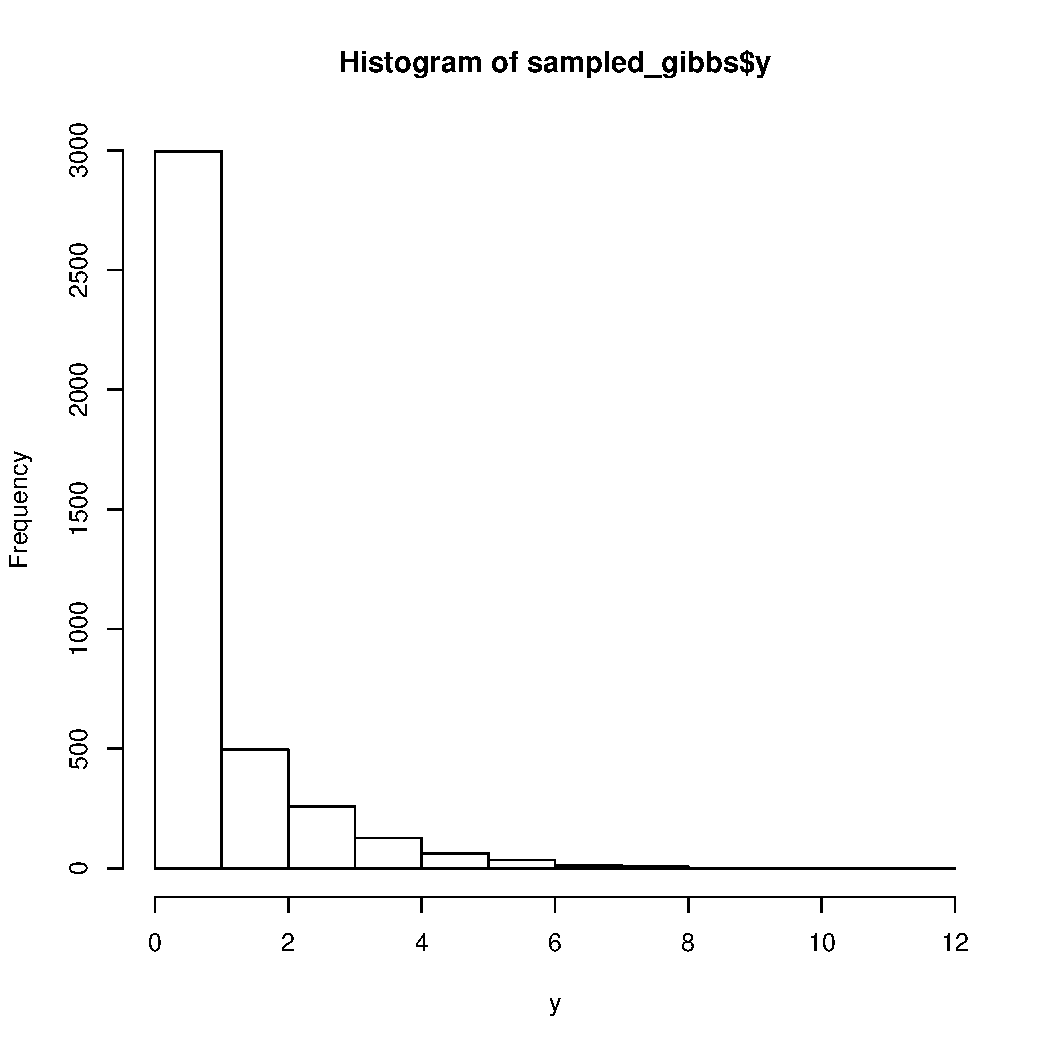
\includegraphics[width=0.60\linewidth]{figure/unnamed-chunk-3-2} 
\begin{kframe}\begin{alltt}
\hlkwd{mean}\hlstd{(sampled_gibbs}\hlopt{$}\hlstd{y)}
\end{alltt}
\begin{verbatim}
## [1] 0.9925
\end{verbatim}
\end{kframe}
\end{knitrout}
$E(Y)=$0.9925, which is very close to the value of the mean of $gamma(1,1)$ Since the x values were derived from that distribution, it would make sense that the average lambda value supplied to y is close to one.
\section*{Exercise 5}
\begin{knitrout}
\definecolor{shadecolor}{rgb}{0.969, 0.969, 0.969}\color{fgcolor}\begin{kframe}
\begin{alltt}
\hlkwd{library}\hlstd{(MCMCpack)}
\end{alltt}


{\ttfamily\noindent\itshape\color{messagecolor}{\#\# Loading required package: coda}}

{\ttfamily\noindent\itshape\color{messagecolor}{\#\# Loading required package: MASS}}

{\ttfamily\noindent\itshape\color{messagecolor}{\#\# \#\#\\\#\# \#\# Markov Chain Monte Carlo Package (MCMCpack)}}

{\ttfamily\noindent\itshape\color{messagecolor}{\#\# \#\# Copyright (C) 2003-2016 Andrew D. Martin, Kevin M. Quinn, and Jong Hee Park}}

{\ttfamily\noindent\itshape\color{messagecolor}{\#\# \#\#\\\#\# \#\# Support provided by the U.S. National Science Foundation}}

{\ttfamily\noindent\itshape\color{messagecolor}{\#\# \#\# (Grants SES-0350646 and SES-0350613)\\\#\# \#\#}}\begin{alltt}
\hlstd{beta_blockers} \hlkwb{<-} \hlkwd{read.csv}\hlstd{(}\hlstr{"g.csv"}\hlstd{)}
\hlstd{beta_blockers} \hlkwb{=} \hlstd{beta_blockers[beta_blockers}\hlopt{$}\hlstd{center} \hlopt{==} \hlnum{1}\hlstd{,]}
\hlstd{beta_blockers}\hlopt{$}\hlstd{death} \hlkwb{<-} \hlnum{1}
\hlstd{beta_blockers}\hlopt{$}\hlstd{death[beta_blockers}\hlopt{$}\hlstd{value} \hlopt{!=} \hlstr{"Death"}\hlstd{]} \hlkwb{=} \hlnum{0}
\hlstd{beta_blockers}\hlopt{$}\hlstd{trt} \hlkwb{=} \hlkwd{as.factor}\hlstd{(beta_blockers}\hlopt{$}\hlstd{trt)}
\hlstd{mc_posterior} \hlkwb{=} \hlkwd{MCMClogit}\hlstd{(death}\hlopt{~}\hlstd{trt}\hlopt{+}\hlstd{ob,} \hlkwc{data} \hlstd{= beta_blockers)}
\hlkwd{summary}\hlstd{(mc_posterior)}
\end{alltt}
\begin{verbatim}
## 
## Iterations = 1001:11000
## Thinning interval = 1 
## Number of chains = 1 
## Sample size per chain = 10000 
## 
## 1. Empirical mean and standard deviation for each variable,
##    plus standard error of the mean:
## 
##                 Mean     SD Naive SE Time-series SE
## (Intercept)  6.06317 4.6184 0.046184       0.250883
## trtT        -0.06891 2.4006 0.024006       0.092080
## ob          -0.13856 0.1035 0.001035       0.005508
## 
## 2. Quantiles for each variable:
## 
##                 2.5%     25%     50%      75%   97.5%
## (Intercept) -0.04411  2.7965  5.0422  8.21607 17.5936
## trtT        -4.62908 -1.6543 -0.1683  1.47173  4.9107
## ob          -0.40264 -0.1868 -0.1122 -0.06347 -0.0144
\end{verbatim}
\begin{alltt}
\hlkwd{plot}\hlstd{(mc_posterior)}
\end{alltt}
\end{kframe}
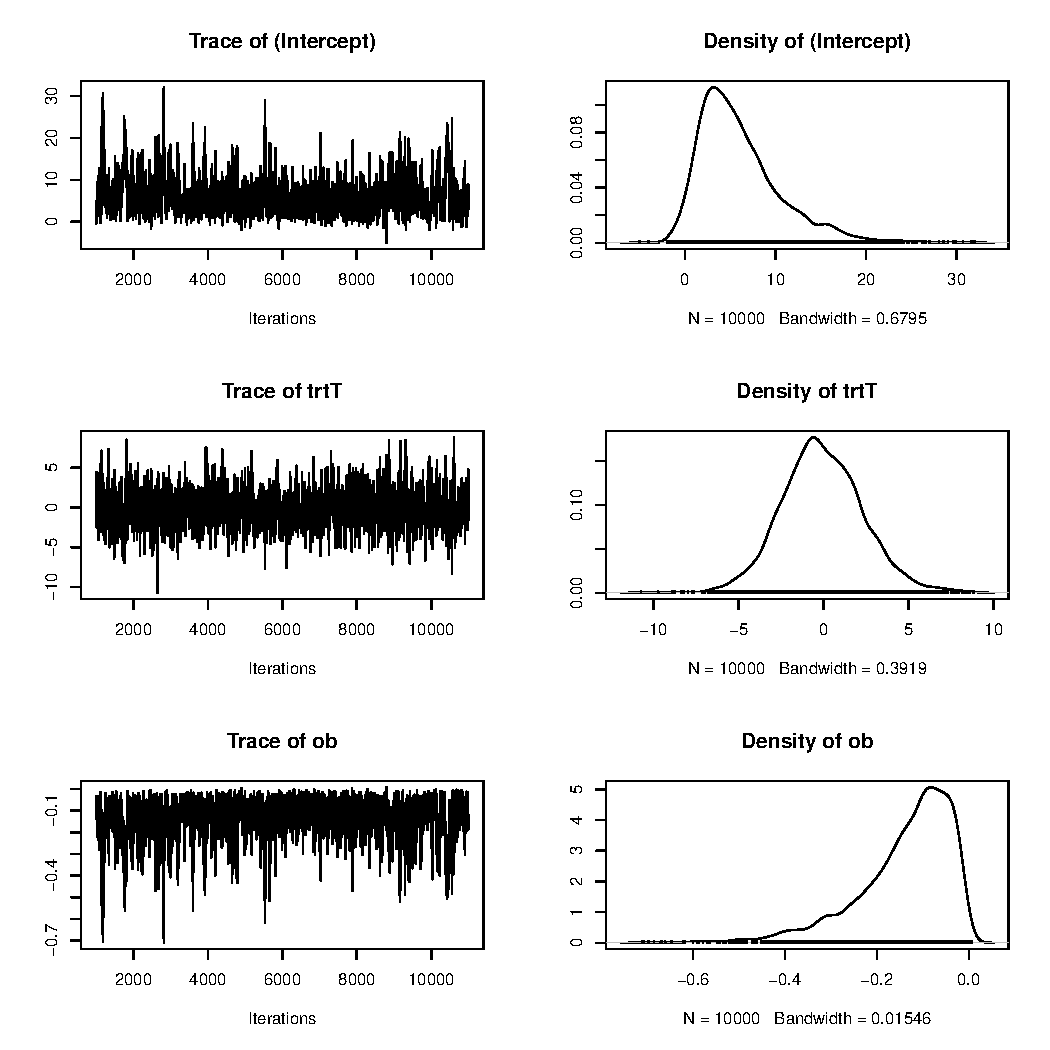
\includegraphics[width=0.60\linewidth]{figure/unnamed-chunk-4-1} 

\end{knitrout}
\end{document}
